\section{ニコ書を支える東京洋菓子倶楽部}

ニコ書チームは、なにかイベントがあるたびに(むしろイベントを無理やり見つけて)、
ホールケーキを買ってきてみんなで食べます。
浜町時代は、明治座の近くにある
東京洋菓子倶楽部\footnote{http://www.yougashi-club.com/}
をよく利用していました。

\begin{figure}[H]
\centering
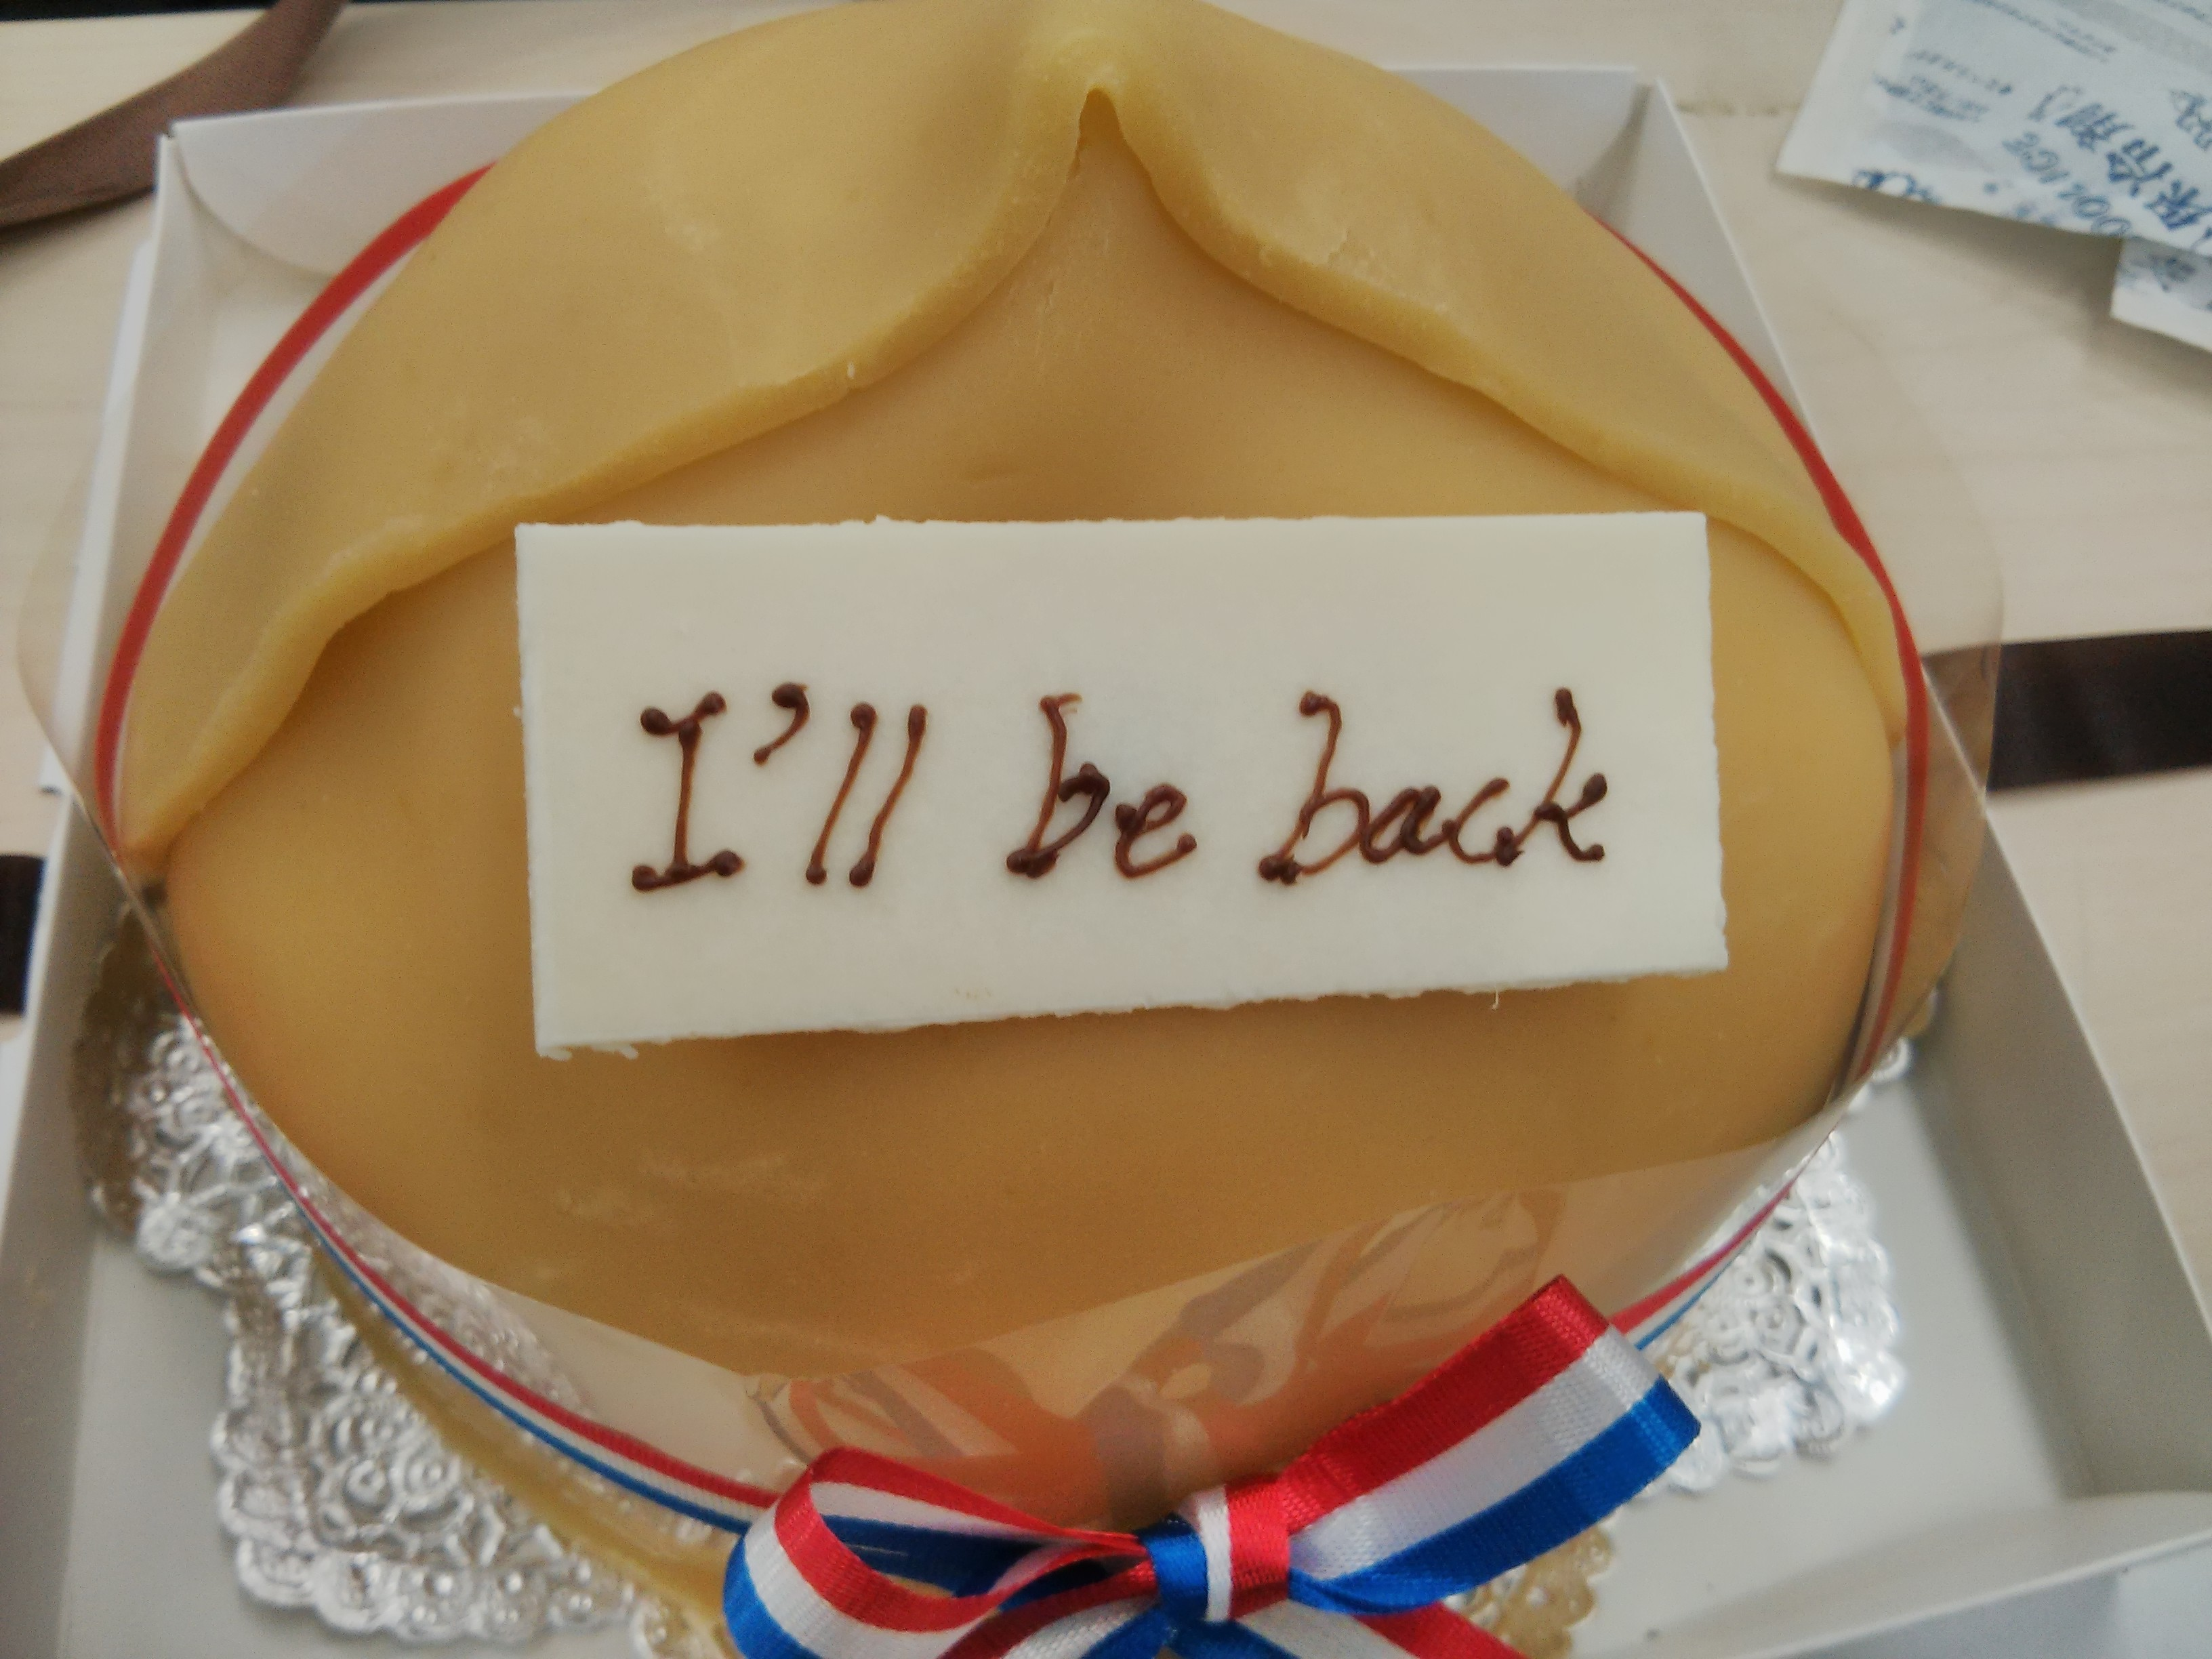
\includegraphics[width=0.7\textwidth]{../images/tokyo_yogashi.jpg}
\caption{名物のモンブラン}
\end{figure}

誕生日を祝うことはもちろん、新しいメンバーの歓迎や転職で去る人へのズッ友会、
人だけでなくリリースの記念や売上記録更新、「システム管理者感謝の日」など、
様々な理由を見つけてはケーキで祝います。
悪ノリが過ぎて他チームの人や転職した人の誕生日を本人不在で祝ったりもしました。

男たちのケーキのくい方は豪快そのもので、ホールケーキを包丁で切ったりなんかしません。
まず最初に祝われる本人がフォークで一口食べます。 それを見届けた後
「よし食え!」 の合図と共に、
全員がフォークを突き立て、突き崩し、奪いあうように貪り食います。
せっかくの美しいケーキが獣たちに蹂躙されます。
レイプ目になったケーキが見えます。

\subsection{プレート}

ホールケーキと言ったらメッセージプレートは必須ですよね。
もちろん「お誕生日おめでとう」なんてつまらないプレートを発注するわけがありません。
祝われる人のキャラクター、祝われる名目、祝われる状況、様々なことを考慮して、
もっとも皮肉の効いたメッセージを用意します。

みんな冗談が通じるメンバーでよかった・・・

\begin{figure}[H]
  \begin{minipage}[t]{0.5\columnwidth}
    \center
    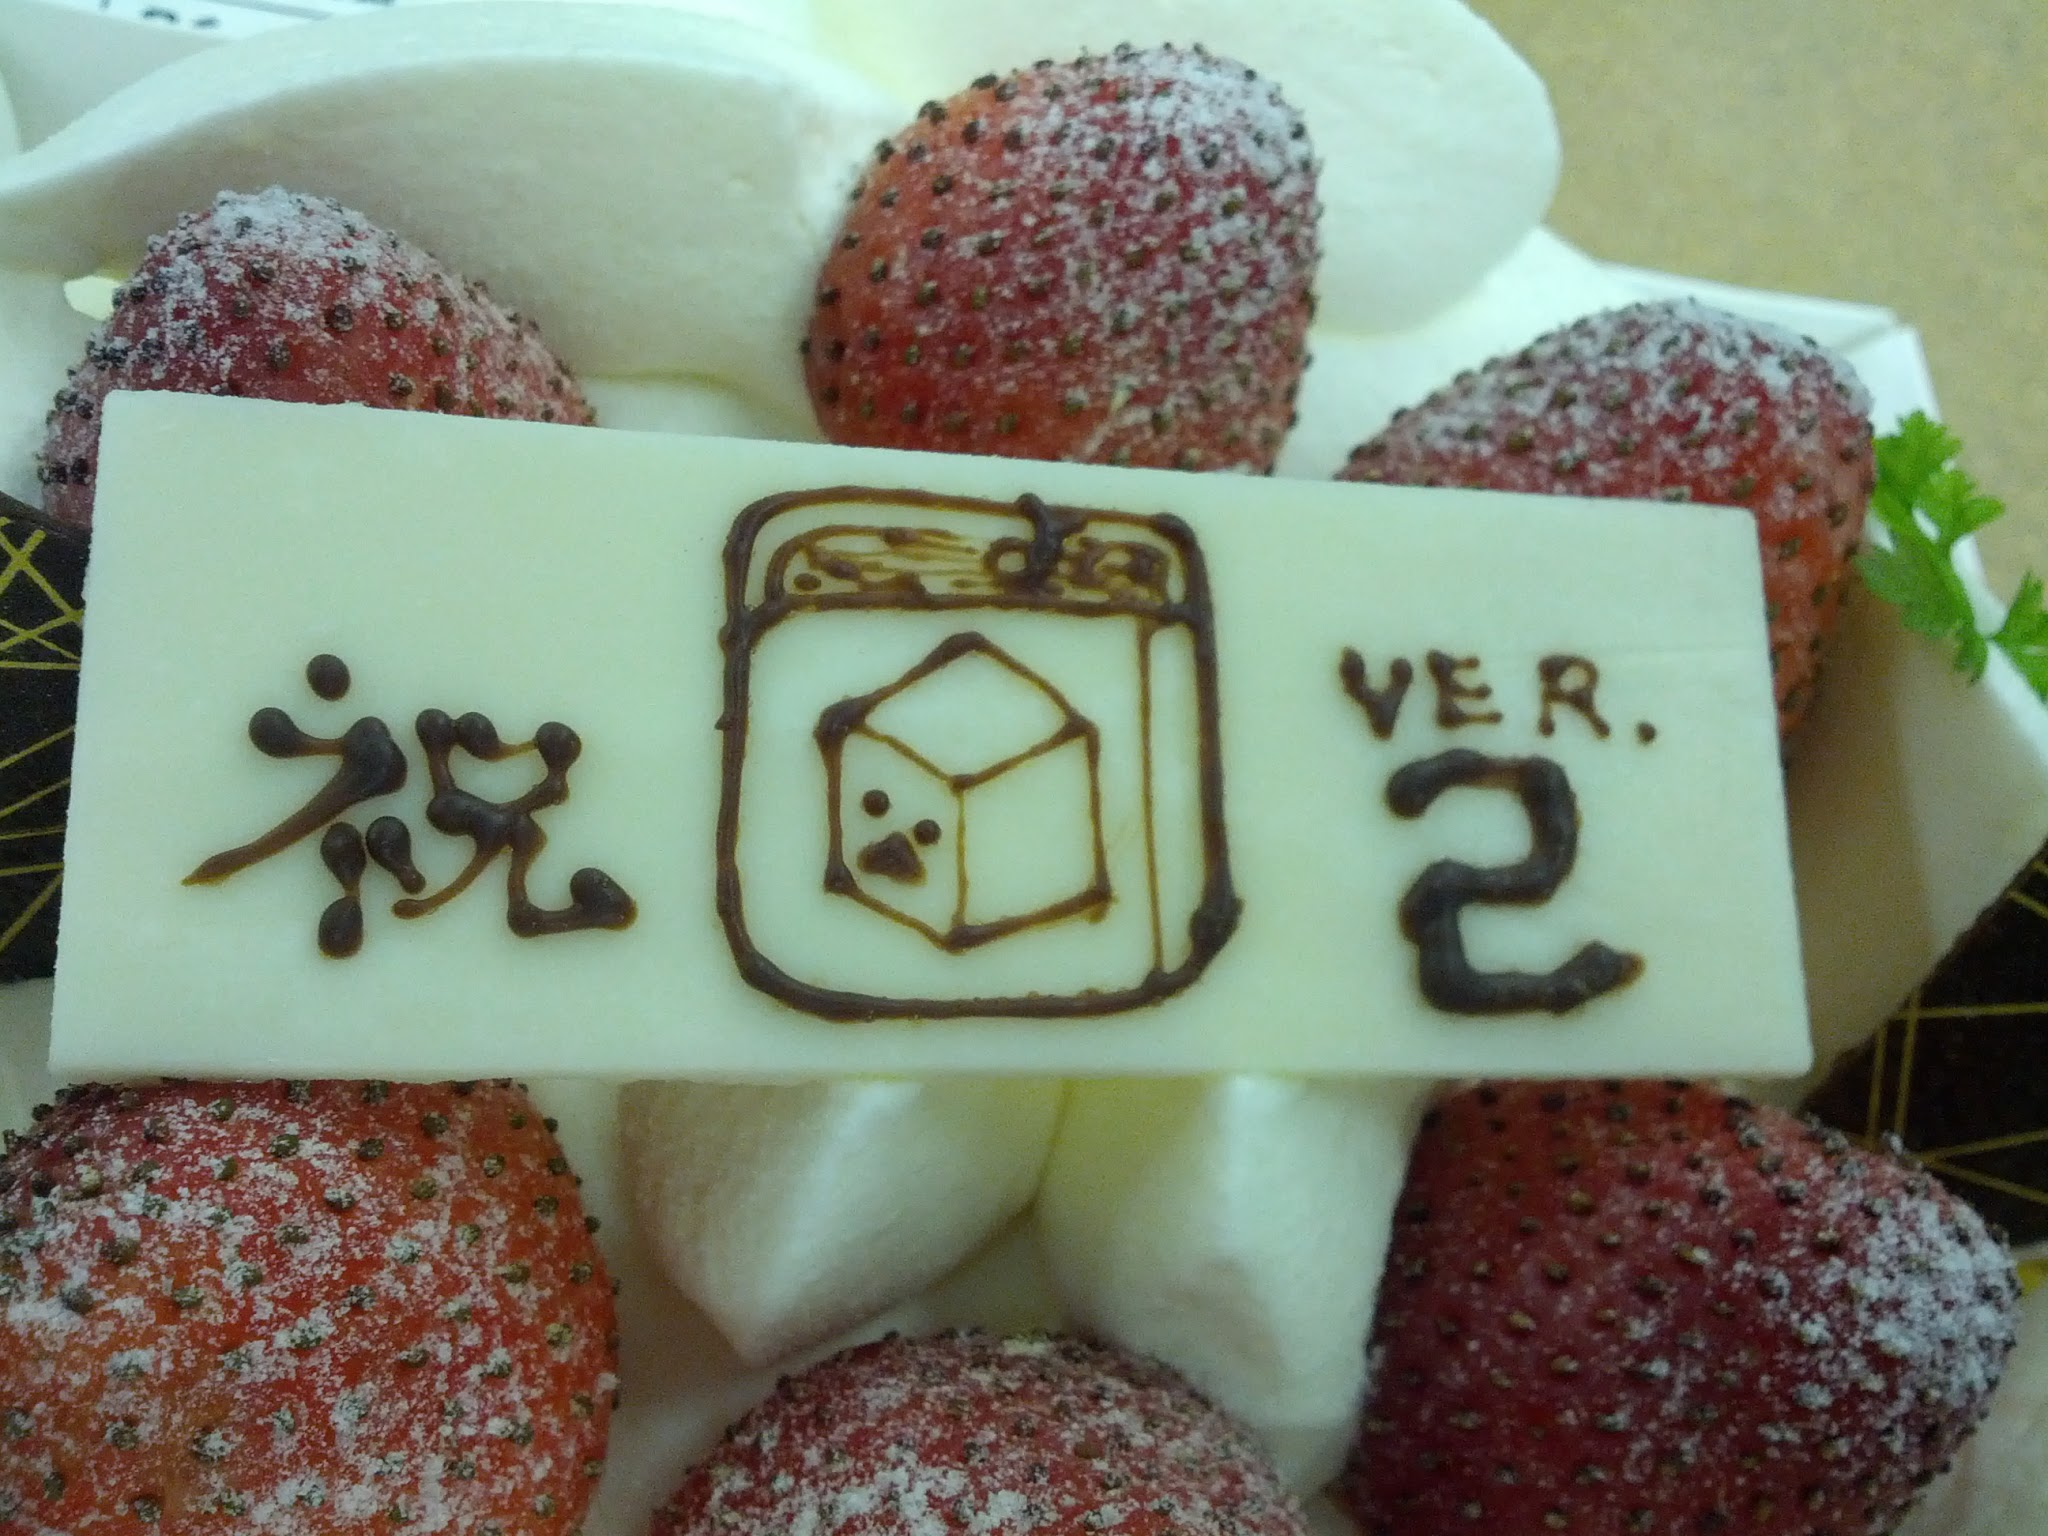
\includegraphics[clip,width=0.9\columnwidth]{../images/cake_ver2.jpg}
    \caption{ios ver.2リリース時のプレート}
  \end{minipage}
  \begin{minipage}[t]{0.5\columnwidth}
    \center
    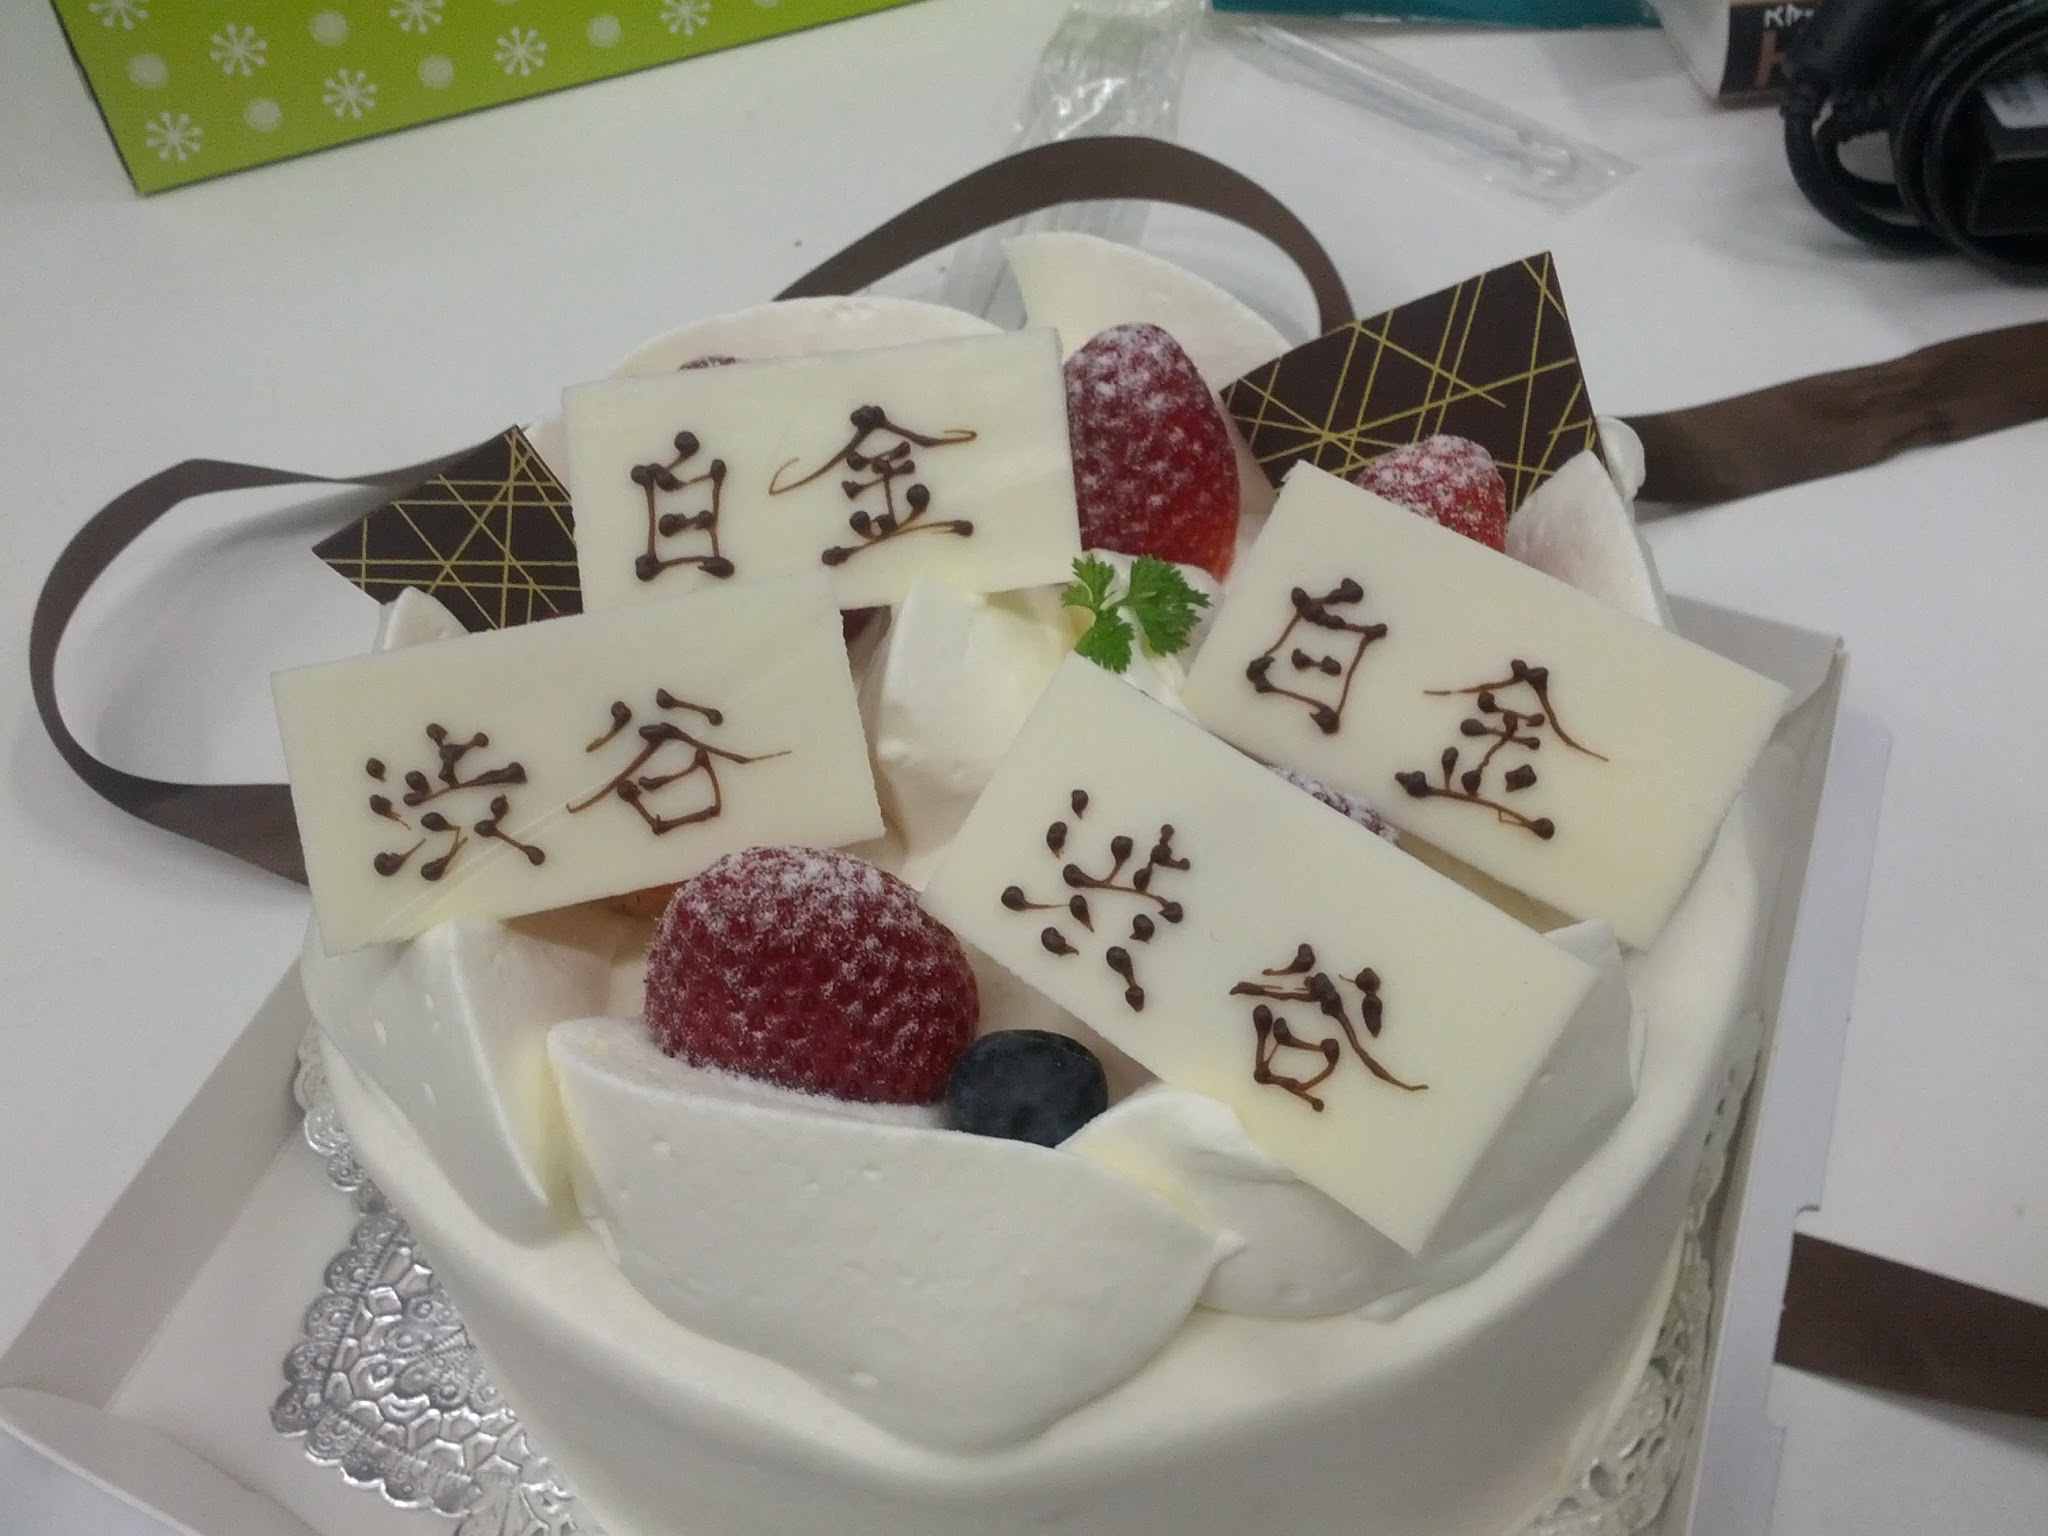
\includegraphics[clip,width=0.9\columnwidth]{../images/cake_4.jpg}
    \caption{4人同時に転職した時のプレート}
  \end{minipage}
\end{figure}

\subsection{アヘ顔ダブルピース}

リア充な会社だとケーキを胸の前に持って満面の笑みで写真を取ってFacebookに載せるんでしょうね。

ニコ書チームはそんなリア充の真似はできないので、
代わりにプレートを口に咥えアヘ顔ダブルピースの写真を撮ります。
そしてFacebookの代わりにニコニコ書籍のdev環境にある「アヘ顔本」に写真を追加していきます。

みんな少しずつアヘ顔がうまくなっていたり、目薬で涙目を演出したり、成長が見られました。

\begin{figure}[H]
\centering
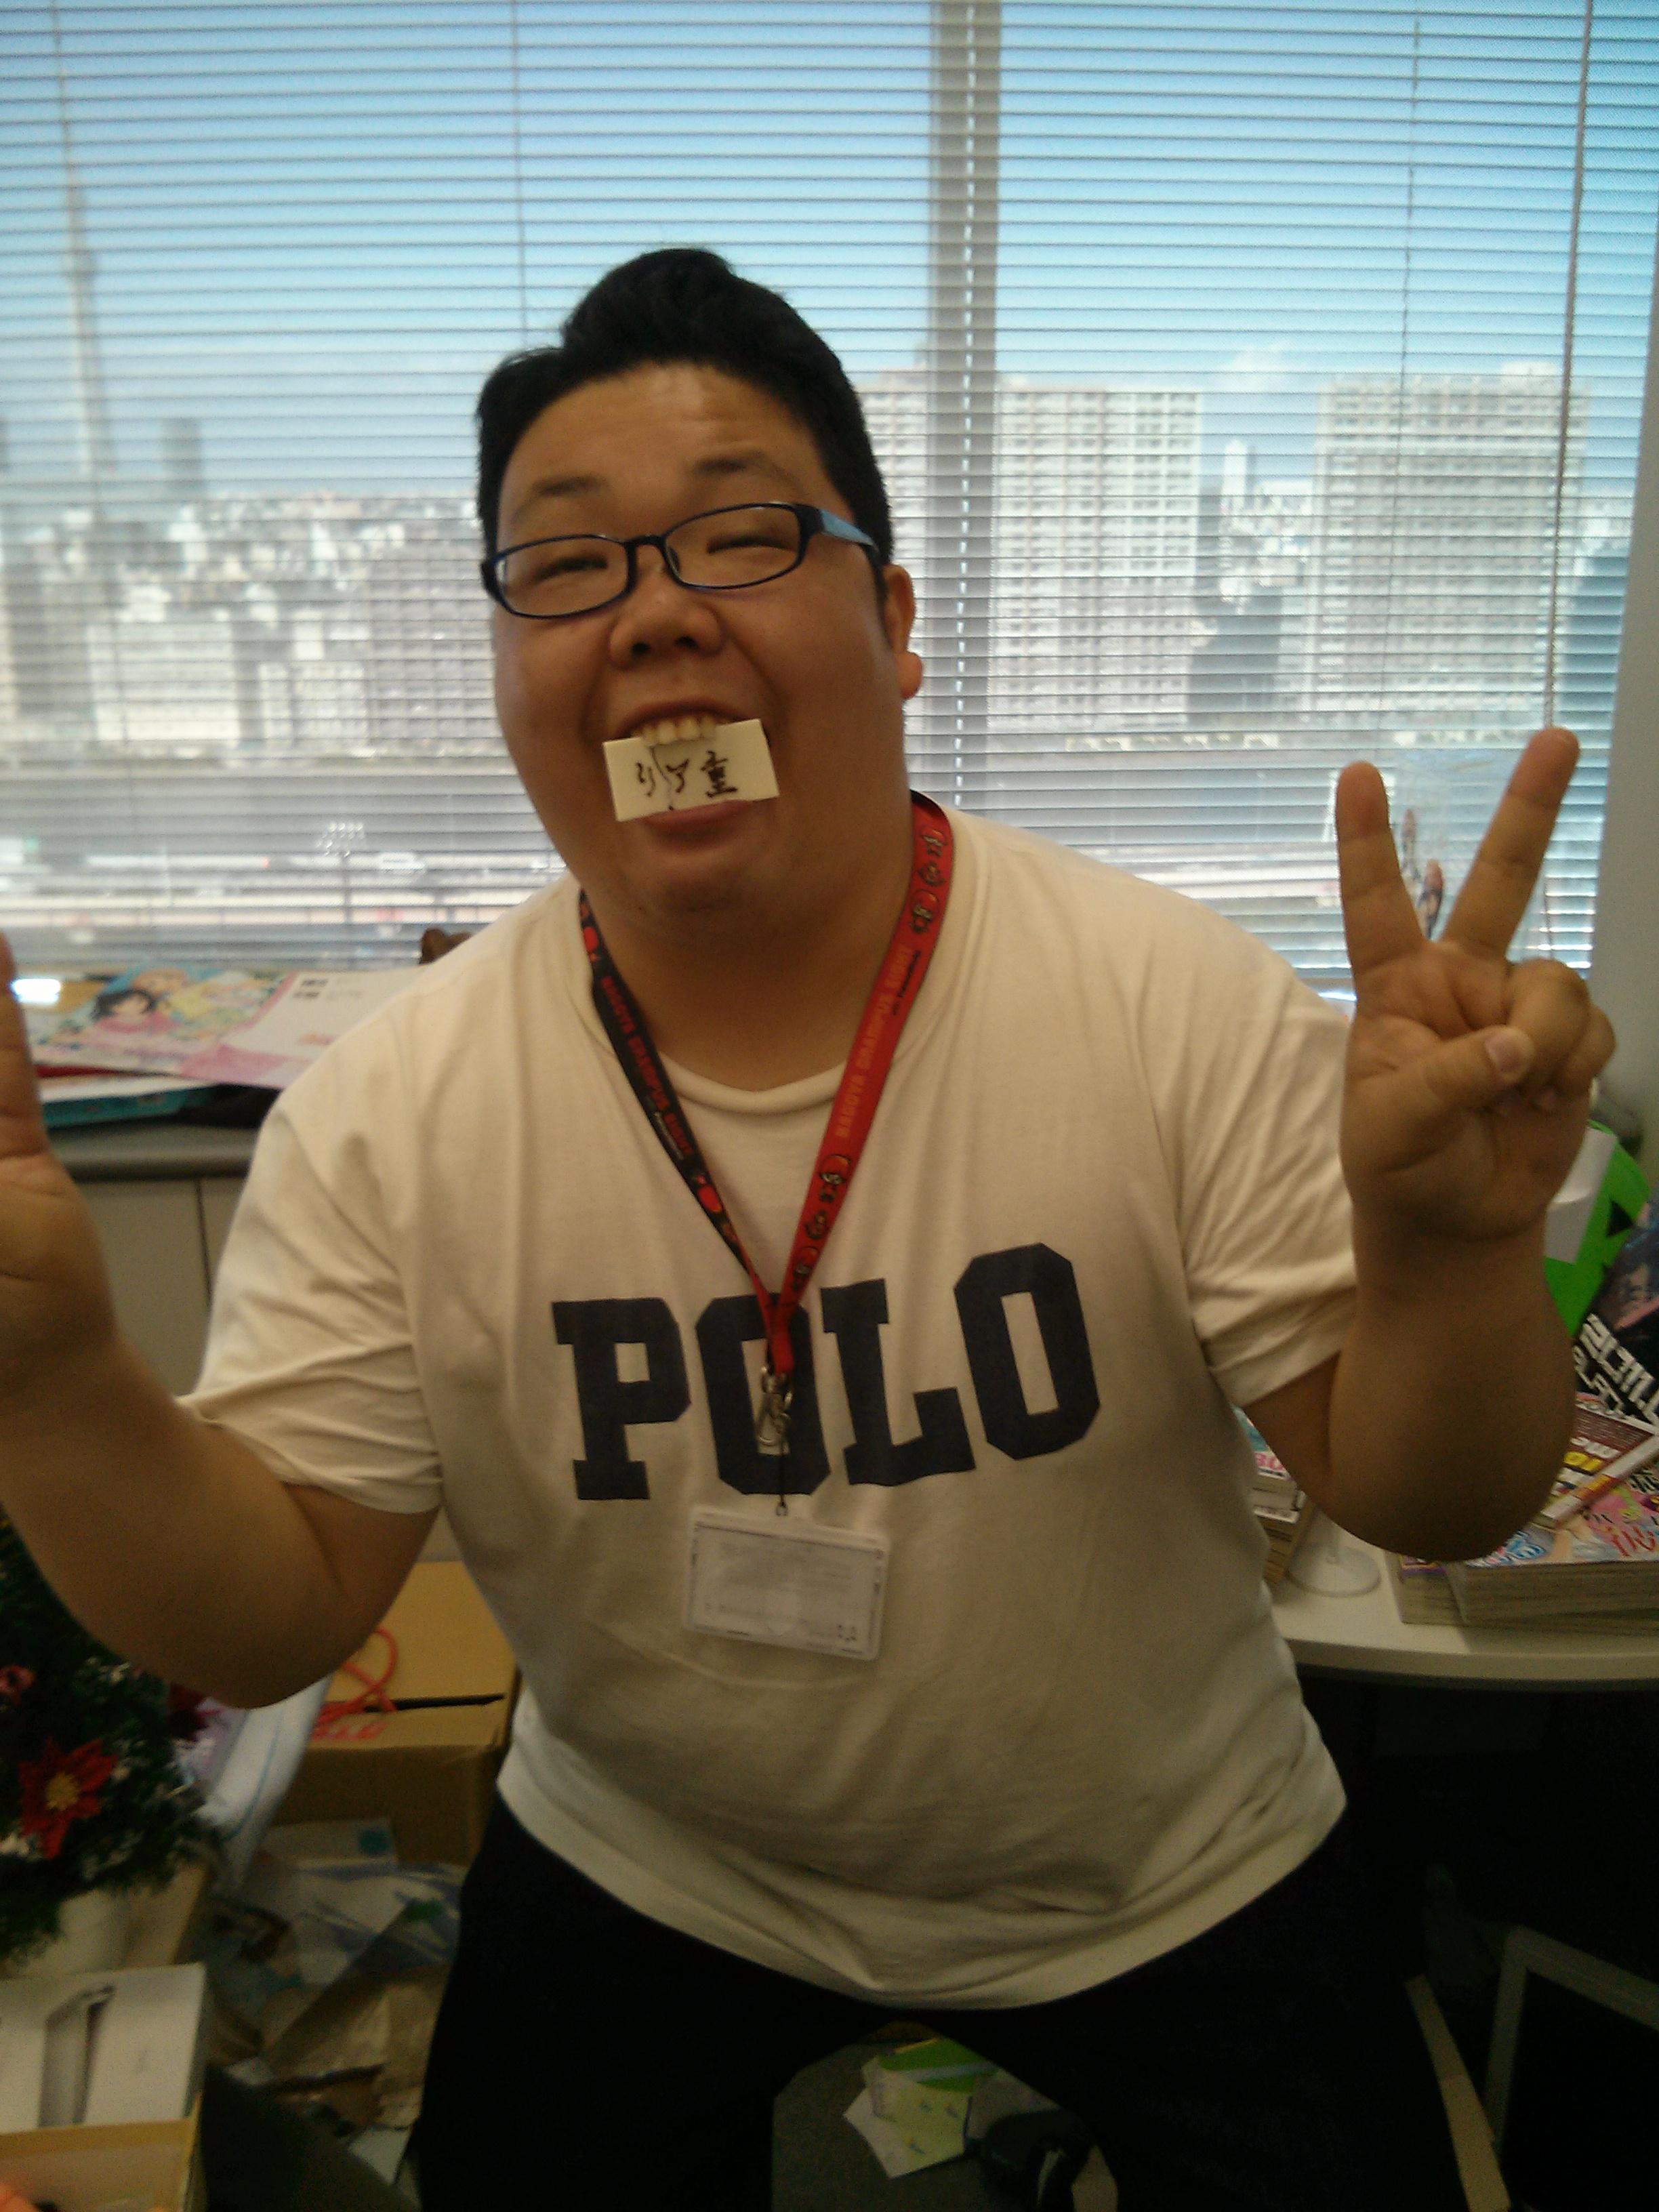
\includegraphics[width=0.6\textwidth]{../images/ahegao_takizawa.jpg}
\caption{tkzwtks初めてのアヘ顔}
\end{figure}

\subsection{ウィッシュリスト}

AmazonのウィッシュリストはWeb業界界隈では随分一般化しましたが、ニコ書チームももちろん活用しています。
この場合も、ただ単にウィッシュリストのものを選ぶだけではなく、
Amazonウィッシュリスト経由で砂1トンを送る方法\footnote{http://data-ssig33.tripod.com/84.html}
 と同じ方法で、主にTENGAなどをバンドルして贈ります。

一度既婚者にTENGAを大量に送ったところ、「こういう男子校のノリ大っ嫌い」と嫁に怒られたそうです。
なお、上記の方法は面倒であろうという配慮から、
最初からウィッシュリストにTENGAを入れておいたところ、
今年の誕生日には技術書と共に40個のTENGAが届きました。


\begin{figure}[H]
\centering
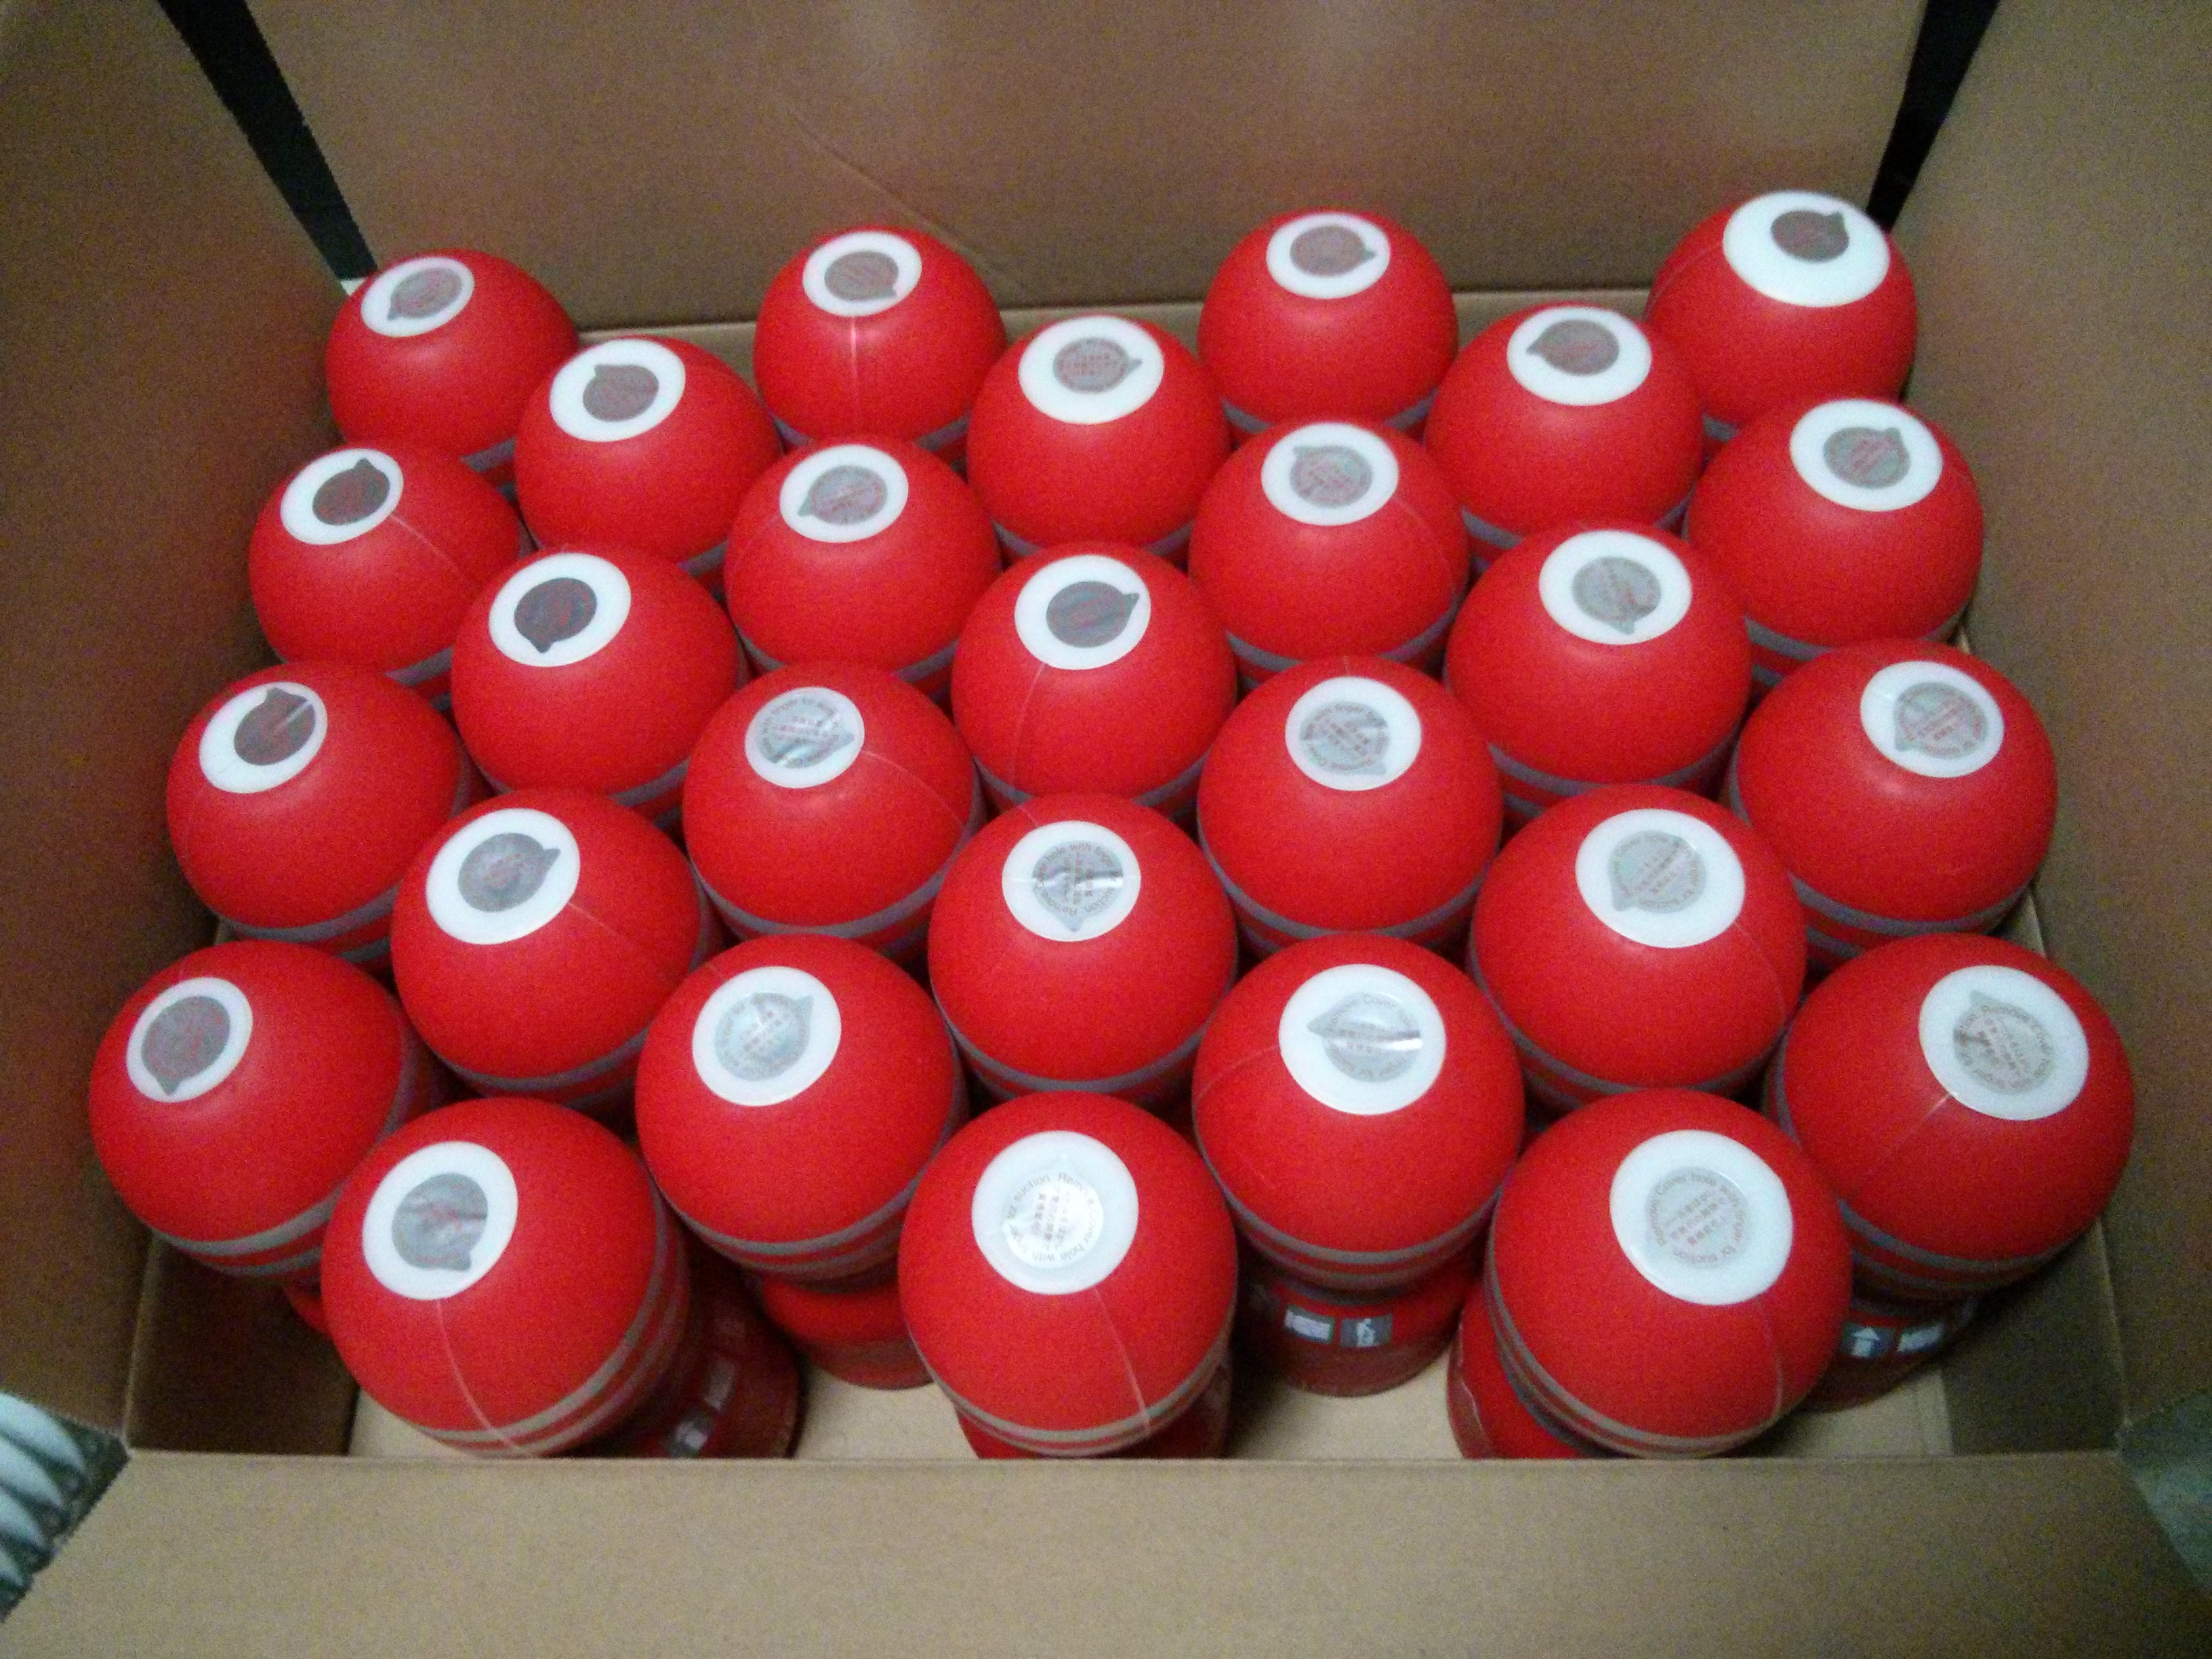
\includegraphics[width=0.6\textwidth]{../images/birthday_tenga.jpg}
\caption{大量に届いたTENGA}
\end{figure}

\subsection{なお}

東京洋菓子倶楽部のケーキは本当に美味しく、
どんなプレートの依頼も予想以上のクオリティで仕上げてくれる、
素晴らしい洋菓子店です。
